% Chapter Template

\chapter{System Design and Architecture} % Main chapter title

\label{Chapter2} % Change X to a consecutive number; for referencing this chapter elsewhere, use \ref{ChapterX}

\lhead{Chapter 2. \emph{System Design and Architecture}} % Change X to a consecutive number; this is for the header on each page - perhaps a shortened title

%----------------------------------------------------------------------------------------
%	SECTION 1
%----------------------------------------------------------------------------------------

\section{Election Data Structure}

\subsection{Skipchains}

The evoting system makes extensive use of a tamper proof blockchain like data structure called Skipchains \cite{skipchains}. An amalgamation of blockchain and skiplists, Skipchains allows clients to traverse forward and backwards in a linear data structure using multi hop links in logarithmic time. As in blockchains, the backward links are cryptographic hashes of the previous blocks. However, the forward links are collective cryptographic signatures of future blocks and are added once the future block is stored.

\begin{figure}[ht]
  \centering
    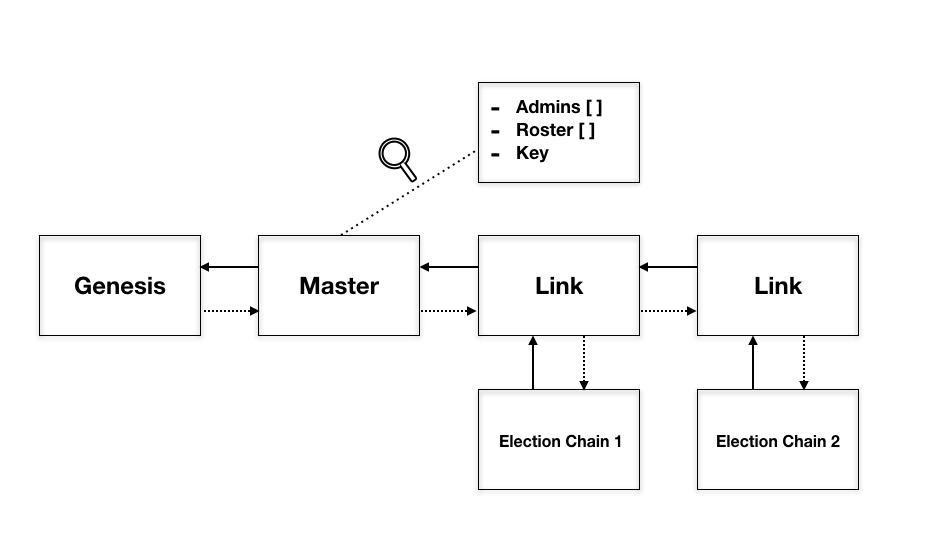
\includegraphics[scale=0.4]{Figures/MasterSkipchain.png}
    \rule{35em}{0.5pt}
  \caption[Master Skipchain]{Master Skipchain}
  \label{fig:MasterSkipchain}
\end{figure}

\subsection{Master Skipchain}

The evoting service is built to support multiple independent elections from the ground up. The global configuration common to a set of elections, and references to those elections themselves are stored in a Skipchain called the Master Skipchain.

Figure \ref{fig:MasterSkipchain} shows an example of a Master Skipchain. The first block, called the genesis block is empty and contains no data. The next block, called the Master Block contains the following configurations

\begin{itemize}
\item Admins: a list of unique 6 digit identifiers for denoting election administrators who may create new elections and finalise them.
\item Roster: a list of servers, called conodes which will participate in the election process.
\item Key: an Ed25519 Public Key used to verify user authentication signature.
\end{itemize}

The remaining blocks, called the election blocks are references to Election Skipchains described in the next subsection.

\subsection{Election Skipchain}

All information associated with a particular election is stored in a sidechain, called the Election Skipchain. The Master Skipchain stores a reference to the genesis block of this sidechain in Link Skipblocks.

\begin{figure}[ht]
  \centering
    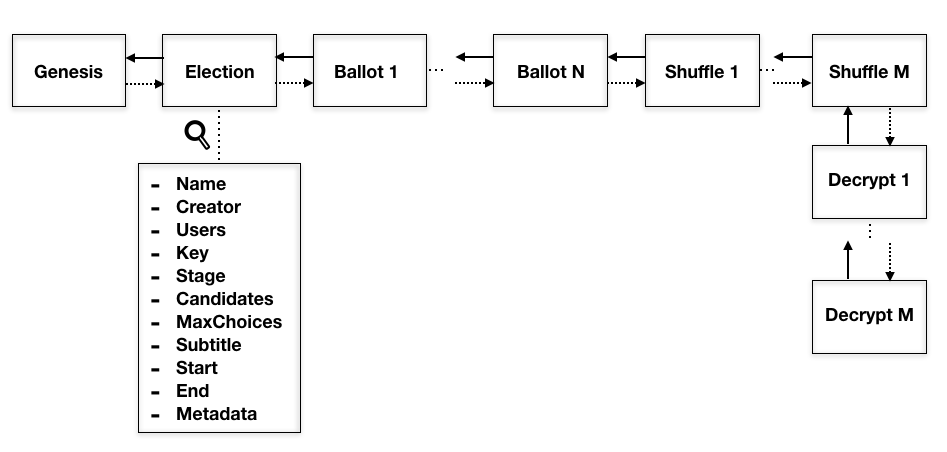
\includegraphics[scale=0.4]{Figures/ElectionSkipchain.png}
    \rule{35em}{0.5pt}
  \caption[Election Skipchain]{Election Skipchain}
  \label{fig:ElectionSkipchain}
\end{figure}

As depicted in Figure \ref{fig:ElectionSkipchain}, the Election Skipchain contains an Election block which stores information associated with the specific election. It contains the following configuration values:

\begin{itemize}
\item Name: Election Title with support for translations in different languages.
\item Creator: Identifier of the administrator who created the election.
\item Users: list of identifiers of users who may vote in this election.
\item Key: an aggregate public key generated using the DKG Protocol \cite{dkg}, which is used to encrypt the ballots.
\item Stage: the current status of election - it may be Running i.e. users may cast their vote, shuffled i.e. the ballots have been mixes or Decrypted i.e. the ballots have been partially decrypted by participating nodes
\item Subtitle: Election Subtitle with support for translations in different languages
\item Start: Timestamp to denote the start of election
\item End: Timestamp to denote end of election
\item Metadata: other keys which store metadata related to the election
\end{itemize}

After the Election Block, the election skipchain consists of a series of Ballot blocks which are stored whenever a user casts a vote. The contents of the Ballot Block include an encrypted ElGamal Ciphertext using the Election Key described above. The user's ballot is encoded in a random point, say $m$ on the Ed25519 Curve \cite{ed25519}. The encryption algorithm then proceeds as follows:

\begin{enumerate}
  \item Alice picks a random \( x \in \mathbb{Z}_{n} \) and computes \( y = gx \). Let $x$ be Alice's secret key and $y$ be her public key.
  \item Bob encrypts a message \( m \in \langle g \rangle \) by selecting a random value \( r \in \mathbb{Z}_{n} \) and computing \( u = gr \) and \( v= m + yr \).
  \item \( (u, v) \) is the ciphertext sent to Alice.
  \item Alice may decrypt the message by recomputing the secret \( s = ux = grx = yr \) and extracts the message with \( m = v - s = m + yr - yr \).
\end{enumerate}

The Ballot Block also contains an identifier for the user who cast the vote. Since the evoting system allows a user to cast multiple ballots, this field is used to determine the last cast ballot for every user before performing the first shuffle.

Once the election is finalised, the election administrator may initiate the shuffle and decrypt protocol which result in the addition of Shuffle and Decrypt blocks in the skipchain. The Shuffle blocks contain a permutation of last cast ballot by every user which participated in the election and a verifiable proof of the mix which is verified by a threshold number of nodes before the block is stored in the skipchain. The decrypt blocks are partial decryptions performed by a threshold number of participating nodes on the ballot encryption contained in the last shuffle block.

\section{Architecture}

\begin{figure}[ht]
  \centering
    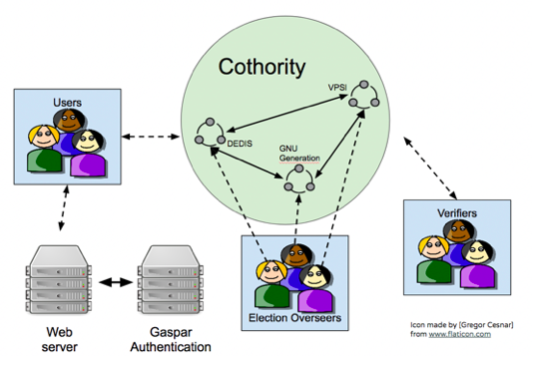
\includegraphics[scale=0.6]{Figures/Architecture.png}
    \rule{35em}{0.5pt}
  \caption[Architecture]{Architecture}
  \label{fig:Architecture}
  \source{Linus Gasser}
\end{figure}

The implementation can be divided into three different components

\begin{enumerate}
  \item A web server that serves static HTML and Javascript files that make up the frontend client.
  \item A web server that acts as an intermediary to authenticate a user against EPFL’s authentication system.
  \item A set of servers, called a \textit{cothority}, with each individual server called a \textit{conode}, which are responsible for handling various protocols associated with the election in a distributed manner.
\end{enumerate}

\subsection{Frontend Webserver}
The frontend server is responsible for serving static HTML and Javascript files to the client. This can be done using any appropriate web server like Nginx \cite{nginx}. The frontend client configuration contains a reference to the Hash of the Master Skipchain and is used to fetch the list of all elections a user may participate in.

\subsection{Authentication Server}
The authentication server is a Node.js \cite{nodejs} webserver that facilitates authentication between the user and Tequila, EPFL’s authentication service \cite{tequila}. Tequila allows users to authenticate with the following protocol

\begin{enumerate}
  \item The service sends a POST request to Tequila with the service’s name, redirection URL and requested parameters as the payload. Tequila then replies with a \textit{urlaccess} token.
  \item The service then redirects the user to Tequila. The \textit{urlaccess} token retrieved before is appended as a query parameter to the GET request
  \item Tequila verifies the user details on submission and redirects the user to the redirection URL for the specified \textit{urlaccess} token irrespective of whether the authentication succeeds or not
  \item The service must then send another POST request to Tequila with the \textit{urlaccess} token as a payload. Tequila replies with the user details and parameters requested in the initial request if the authentication was successful or an error is returned otherwise.
\end{enumerate}

It should be noted that as of now Tequila only allows verifying the \textit{urlaccess} token mentioned in the last step of the protocol only once. Any further attempts to validation results in an error being returned. In our context, the authentication server acts as the service that interacts with Tequila. On confirmation of successful authentication of the user from Tequila, the authentication server generates a Schnorr signature which is stored in the browser’s localStorage \cite{localStorage}. This signature is used to verify all transactions as described in the next subsection about Cothority.

\subsection{Cothority}

A collective authority or cothority \cite{cothority} is a set of nodes that witness a particular transaction in a Skipchain and a threshold number of nodes collectively authorise it to be stored. The framework is a research project at the DEDIS laboratory at EPFL, allowing easy deployment of decentralised and distributed services and protocols. The conodes participating in the election run the evoting and skipchain service for orchestrating the elections and storing the data in skipchains respectively.

The skipchain service in cothority allows execution of a verifier function which is run by all the participating nodes in the election roster. All transactions that write data to the skipchain have user identity verification as a part of the verification function. This user identification involves validating the  Schnorr signature of the concatenation of user's identifier (sciper) and the Master Skipchain's Genesis Block Hash against the Authentication Server's public key which is stored in the Master Skipchain's Master Block.

\section{Protocols}

The evoting system runs protocols at different stages of the election process to perform operations in a distributed manner. The cothority framework helps in the implementation and testing of these distributed protocols.

\subsection{Distributed Key Generation (DKG)}
The cothority framework contains an implementation of the Distributed Key Generation (DKG) protocol by Gennaro et. al. \cite{gennaro1999secure}. DKG distributes the secret key over a set of nodes, thereby disallowing any particular server the capability of shuffle or decrypt the ballots.

The protocol begins with each node $N_i$ calculating a secret share $s_i$. This is followed by a series of message exchanges that removes potentially malicious nodes and results in a set of qualified nodes \textit{QUAL}. The aggregate secret $x$ is the sum of all the individual secrets of qualified nodes
$x = \sum_{i \in \textit{QUAL}}s_i$. The corresponding public key can be calculated as $y = gx$. The DKG protocol is executed whenever an election administrator requests a new election to be created. Every participating node generates its secret and the aggregate public key is stored in the newly created election skipchain along with other Election Metadata. It is this public key which is used by the frontend client to encrypt the user ballots. The protocol is initialised with a threshold that requires at least \( \lfloor\dfrac{2n}{3}\rfloor + 1 \) nodes to reconstruct the decryptions later where $n$ is the total number of nodes in the roster.

\subsection{Shuffle}

Once the election ends, the election creator may initiate the shuffle protocol which re-encrypts, permutes and appends the result on the election skipchain providing a proof of the shuffle. The shuffle protocol proceeds as follows:

\begin{enumerate}
  \item The protocol begins with the leader node being contacted by the client to initiate the shuffle. The leader first checks the presence of a threshold number of shuffles already in the skipchain and exits if so.
  \item In the presence of shuffle blocks lesser than the threshold number required, the leader prepares a list of servers which may participate in this instance of the shuffle, excluding the ones that participated before.
  \item In the first attempt at generating the shuffle, the leader iterates through the election skipchain, finding the last ballot cast by each user and appending it to a list. This list is then passed on as an input to the Neff Shuffle function. On the other hand, other attempts at shuffle rely on the last shuffle that is stored in the skipchain and use it as the input to the Neff Shuffle function.
  \item The Neff Shuffle function then permutes the ballots and outputs a permuted list of ballots and a corresponding proof. The node which created the permutation requests the storage of the shuffle which must be ratified by a threshold of participating conodes in the election. In order to ascertain its identity, the node also signs its public key and stores it as a part of the block data along with its public key in clear text.
  \item On receiving a request to store the shuffle block, the  participating nodes verify the identity of the node which proposed the shuffle by checking the signature of the public key included in the transaction. They then ensure that the election skipchain does not already have a threshold number of shuffle blocks and the node which has proposed the given shuffle has not stored a shuffle previously. The nodes then run the Neff Shuffle proof verifying the integrity of the shuffle. If all these checks are ratified by a threshold number of participating nodes the shuffle is stored in the skipchain
  \item The proposer then requests the next server in the list to repeat the shuffle until we get a threshold number of shuffles in the skipchain or the protocol times out.
\end{enumerate}

It should be noted that the shuffle protocol is resilient to failures due to non availability of nodes and timeouts. At every attempt, the protocol tries to pick off from the point where it was abandoned.

\subsection{Decrypt}

The decrypt protocol is used to store a threshold number of partial decryptions by the participating nodes. The protocol proceeds as follows:

\begin{enumerate}
  \item The protocol begins with the leader node being contacted by the client to initiate the decryption. The leader first checks the presence of a threshold number of decryptions already in the skipchain and exits if so.
  \item In the presence of partial decryptions lesser than the threshold number required, the leader prepares a list of servers which may participate in this instance of the decrypt protocol, excluding the ones that participated before.
  \item The leader then sends a broadcast to the whitelisted servers and prompts them to partially decrypt the last shuffle stored in the skipchain using their share of the private secret generated during the DKG protocol.
  \item Every node tries to store their partial shuffle on the skipchain. The participating nodes run the verification function which checks if the election skipchain has threshold number of shuffles in place, verifies the identity of the proposing node by checking the signature of its public key included in the transaction, checks if the node has not stored a partial decryption before.
  \item If all the checks pass, the shuffle is stored on the skipchain. The node then sends a reply back to the leader indicating success or failure.
  \item The leader maintains a count of successful partial decryptions and ends the protocol as soon as a threshold number of success messages are received.
 \end{enumerate}
 
 Like the shuffle protocol, the decrypt protocol is also resilient to failure due to non availability of nodes and timeouts. Every reinitialisation of the protocol results in an attempt to pick off from the previous failed attempt.
